\begin{figure}[htbp]
  \centering
  \begin{tabular}{ccc}
    \begin{minipage}{0.33\hsize}
      \includegraphics[width=4cm]{../pic/Run78/BL/BLC1_time.eps}
    \end{minipage}
    \begin{minipage}{0.33\hsize}
      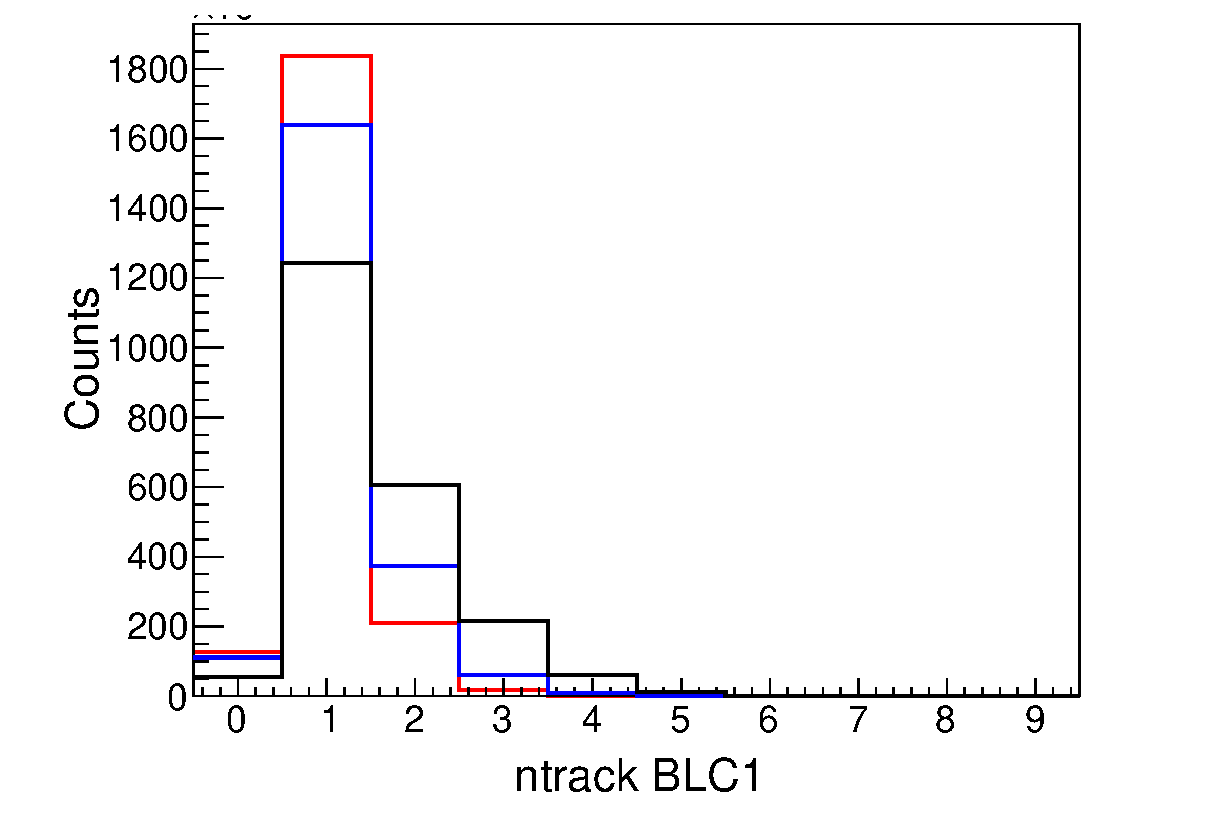
\includegraphics[width=4cm]{../pic/Run78/BL/nBLC1.eps}
    \end{minipage}
    \begin{minipage}{0.33\hsize}
      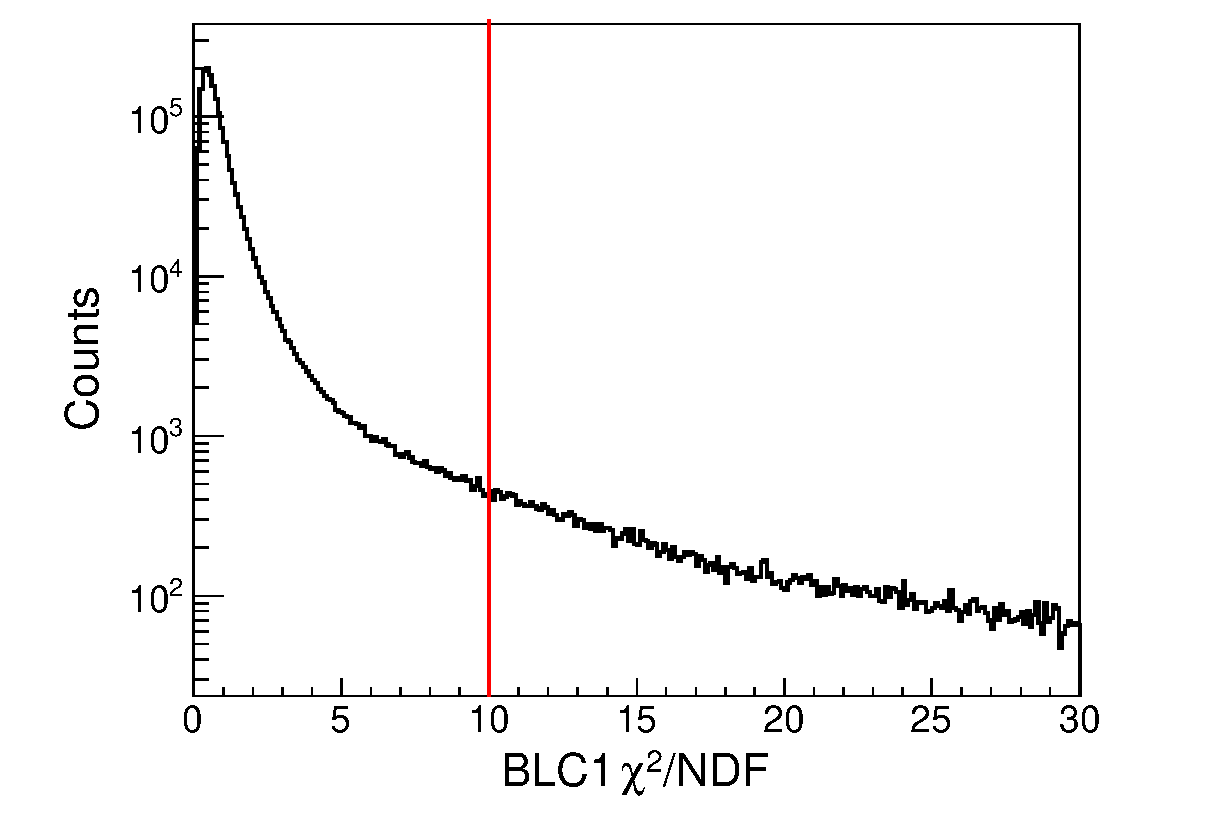
\includegraphics[width=4cm]{../pic/Run78/BL/BLC1_chi2.eps}
    \end{minipage}
  \end{tabular}

  \begin{tabular}{ccc}
    \begin{minipage}{0.33\hsize}
      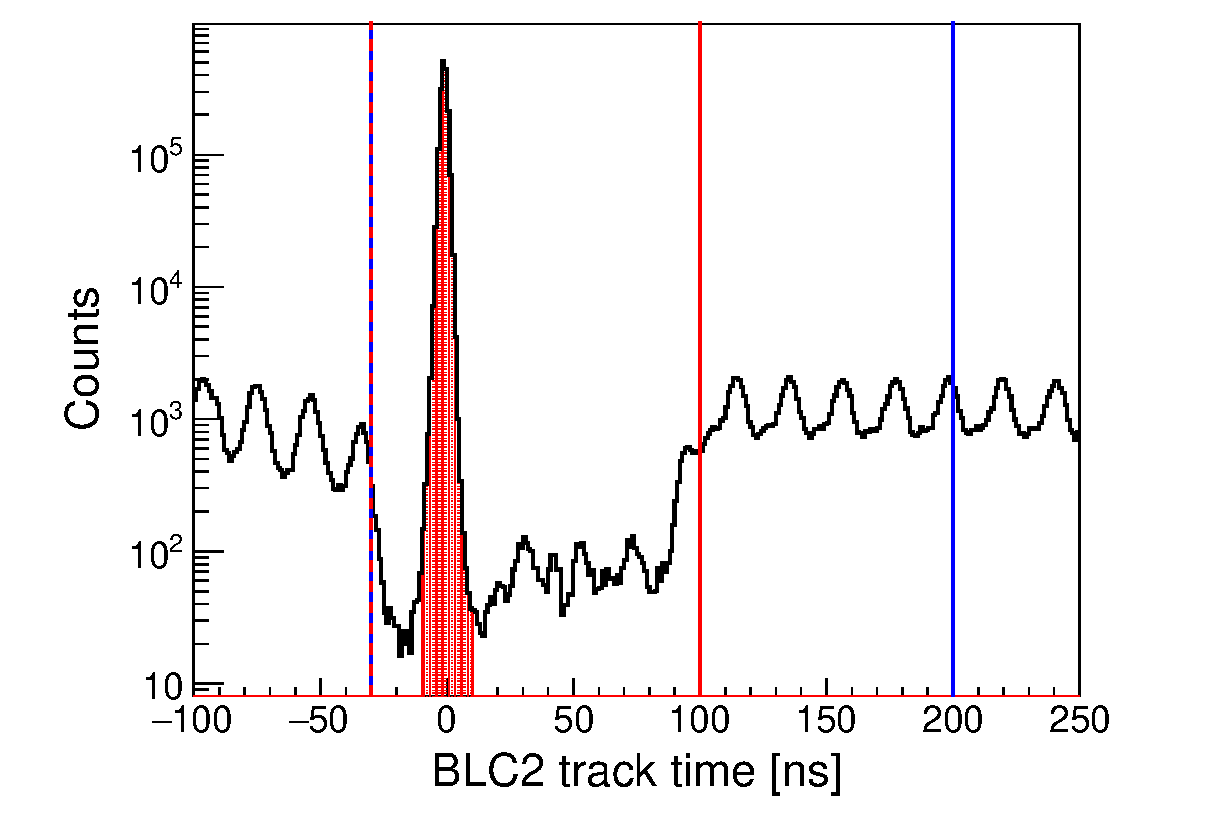
\includegraphics[width=4cm]{../pic/Run78/BL/BLC2_time.eps}
    \end{minipage}
    \begin{minipage}{0.33\hsize}
      \includegraphics[width=4cm]{../pic/Run78/BL/nBLC2.eps}
    \end{minipage}
    \begin{minipage}{0.33\hsize}
      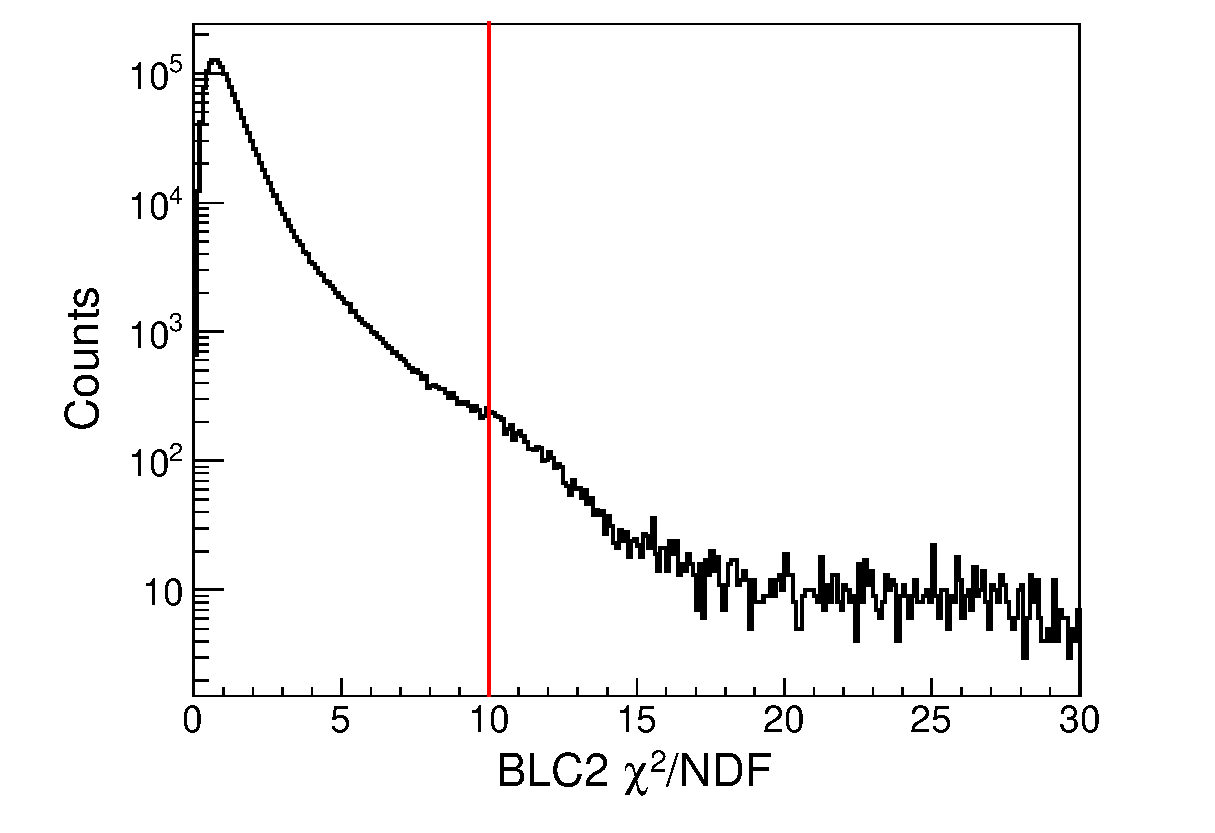
\includegraphics[width=4cm]{../pic/Run78/BL/BLC2_chi2.eps}
    \end{minipage}
  \end{tabular}

    \begin{tabular}{ccc}
    \begin{minipage}{0.33\hsize}
      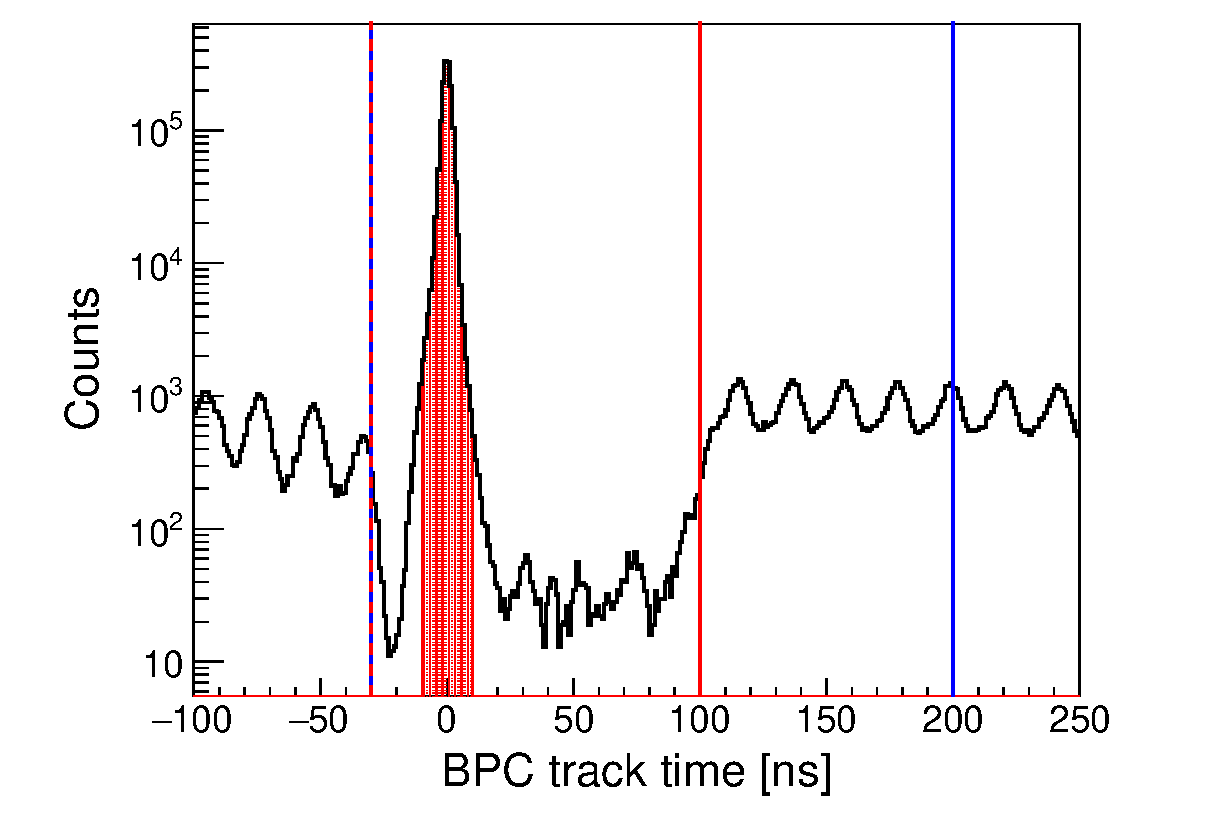
\includegraphics[width=4cm]{../pic/Run78/BL/BPC_time.eps}
    \end{minipage}
    \begin{minipage}{0.33\hsize}
      \includegraphics[width=4cm]{../pic/Run78/BL/nBPC.eps}
    \end{minipage}
    \begin{minipage}{0.33\hsize}
      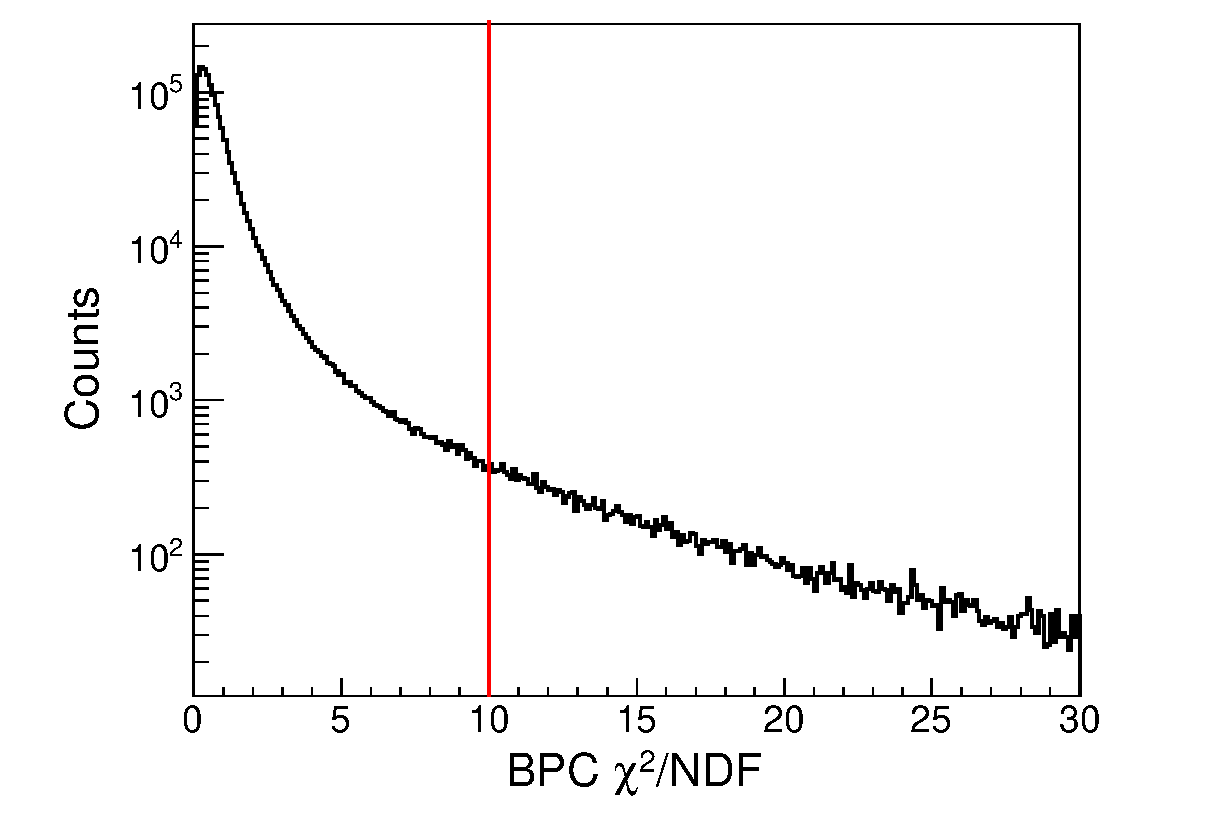
\includegraphics[width=4cm]{../pic/Run78/BL/BPC_chi2.eps}
    \end{minipage}
  \end{tabular}
  \caption{
    The left, the middle and the right figures show the number of tracks, track time and $\chi/NDF$, respectively.
    Color plots in the left figure indicate some time window.
    % Black, blue, red indicate all, $-30\sim200$[ns], $-30\sim100$[ns], respectively.
    The above, the middle and the down figures represent BLC1, BLC2 and BPC, respectively.
    The BPC was described after.
  }
  \label{fig:BLDC_selection}
\end{figure}
